\subsection{Initial analysis}
First, we decided to explore our data with respect to severity, which is useful for our analysis.
\begin{figure}[htpb!]
	\minipage{0.5\textwidth}
	\centering
	\includegraphics[width=1\textwidth]{../imgs/pdf_files/top5deaths.pdf}
	\caption{\textbf{Top categories by deaths}}
	\label{fig:top5d}
	\endminipage
	\hfill
	\minipage{0.5\textwidth}
	\centering
	\includegraphics[width=1\textwidth]{../imgs/pdf_files/top5injuries.pdf}
	\caption{\textbf{Top categories by injuries}}
	\label{fig:top5inj}
	\endminipage
\end{figure}
We can see from figure \ref{fig:top5d} that most of the deaths occur when pedestrians are involved, next deadliest are crashes, obstacle encounter,
crashes with non-moving vehicles, overturns. Nothing surprising. We get similar results for injuries:
\noindent
 Most injuries occur during crashes, pedestrian and obstacle encounters, crashes with non-moving vehicles,
falls of passengers.
Interestingly, if we count number of deaths with respect to total participants by category of accident, we get the results 
as shown in table \ref{tab:prob_death}.
\begin{table}[h]
	\centering
	\label{tab:prob_death}
	\begin{tabular}{|c|c|}
		\hline
		Category & $P_{\text{death}}$ \\
		\hline
		Hitting maintenance worker & 0.23 \\
		\hline
		Crash into ditch & 0.14 \\
		\hline
		Hitting other & 0.12 \\
		\hline
		Hitting police officer & 0.09 \\
		\hline
		Running over animals & 0.09 \\ 
		\hline
		Obstacle encounter & 0.09 \\
		\hline
		Overturn & 0.05 \\
		\hline
		Other type of accident & 0.05 \\
		\hline
	\end{tabular}
	\caption{\textbf{Top 8 Probability of death with respect to accident}}
\end{table}
\noindent
The high mortality rate is not surpising. There are relatively few participants in these types of accidents (less than 130), except obstacle encounter.
All of these events are quite similar in terms of that they mostly happen on motorways, where speeds are high and thus crashes are more lethal when
they occur. However, as we saw from figure \ref{fig:top5d} most deaths occur in habited areas. \\
\subsection[Clusterization]{Clusterization\footnote{\href{https://github.com/isdevnull/cw3/blob/dev/clusters.ipynb}
{https://github.com/isdevnull/cw3/blob/dev/clusters.ipynb}}}
Our data possesses geospatial properties, that is why we decided that it would be nice to explore potentially dangerous areas. There are just too
many accidents in Moscow, so it may seem that they cover almost all of the streets and motorways and in fact it is absolutely true. However,
we can employ density-based clusterization technique to select only those spots on the map that are most dense in terms of car accidents. To do that
we use DBSCAN \cite{DBSCAN}, which can select clusters of complex form, depends only on a few hyperparameters which are easily interpretable.
\begin{figure}[H]
	\centering
	\includegraphics[width=0.8\textwidth]{../imgs/png_files/msc_problem_regions.png}
	\caption{Clusterizaion with U=$\frac{0.1}{6371}$, N=$15$; red points – deadly accidents, purple – heavy severe}
	\label{fig:DBSCAN}
\end{figure}
These are neighbourhood of a point – $U$ and number of members – $N$ to be considered as core point.
Due to Earth being spherical we use Haversine distance and
transform our geospatial data to radians, thus neighbourhood $U$ in our case is distance between multiple accidents and core samples are defined as
those that have $N$ accidents around it, scattered in time. When DBSCAN selects $M$ clusters, we firstly delete noise points, then we do not
distinguish between clusters, because we are only interested, in general, how problematic regions are distributed. We color accidents according
to their severity. The larger the $U$ hyperparameter the bigger the problematic regions and the more spreaded they are.
\subsection{Time Series Analysis}

Because we want to predict severity and it is a categorical variable, we assign label 0 to cases without significant injuries and 1 otherwise.
First of all we examine the behavior of the variable. As we can see the number of severe car accidents declines as shown on figure \ref{fig:ts_sev}.
However as it was mentioned above severity combines two features.
Therefore we plot number of injuries and deaths per month as well.
As we compare two figures \ref{fig:ts_inj} and \ref{fig:ts_death}, it is clear that the downward trend of the number of severe cases can be attributed the the decline of number of deaths.
The graph for injuries(\ref{fig:ts_inj}) heavily fluctuates around its mean, whereas the girth depicting number of deaths declines. 
If we review this graph separately we may notice that beside downward trend it also has a yearly seasonality.
We visualize the behaviour of number of deaths (figure \ref{fig:ts_death}) and compare it to the number of car accidents throughout a day.
The analysis shows (figure \ref{fig:ts_dist}) that the number of accidents peaks at a daytime, however the most risky time for a person is night,
as it is four times more likely to be killed or injured from midnight to 7 a.m. 
Based on that information we construct additional features and estimate their potential to be useful predictors.
Correlation of the newly created predictors is shown below:
\begin{figure}[htpb]
	\centering
	\includegraphics[width=0.5\textwidth]{../imgs/pdf_files/new_embeddings_correlation.pdf}
	\caption{Correlation of embeddings}
	\label{fig:new_embed}
\end{figure}

\begin{figure}[htpb]
	\centering
	\includegraphics[width=0.8\textwidth]{../imgs/pdf_files/ts_severity.pdf}
	\caption{Severity from 01.2015 till 04.2021}
	\label{fig:ts_sev}
\end{figure}

\begin{figure}[htpb]
	\centering
	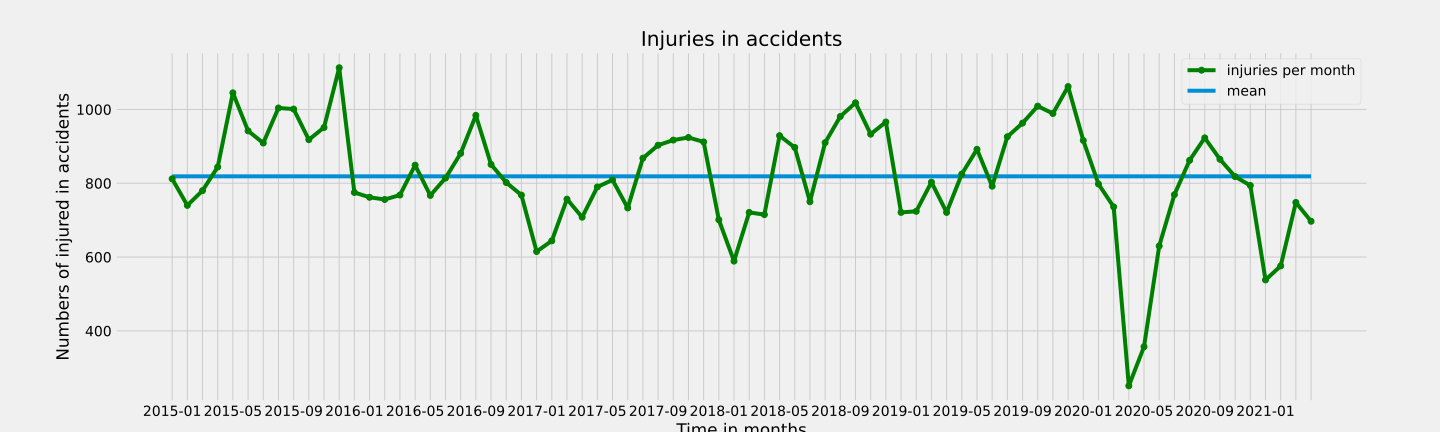
\includegraphics[width=0.8\textwidth]{../imgs/pdf_files/ts_injuries.pdf}
	\caption{Number of injuries from 01.2015 till 04.2021}
	\label{fig:ts_inj}
\end{figure}

\begin{figure}[htpb]
	\centering
	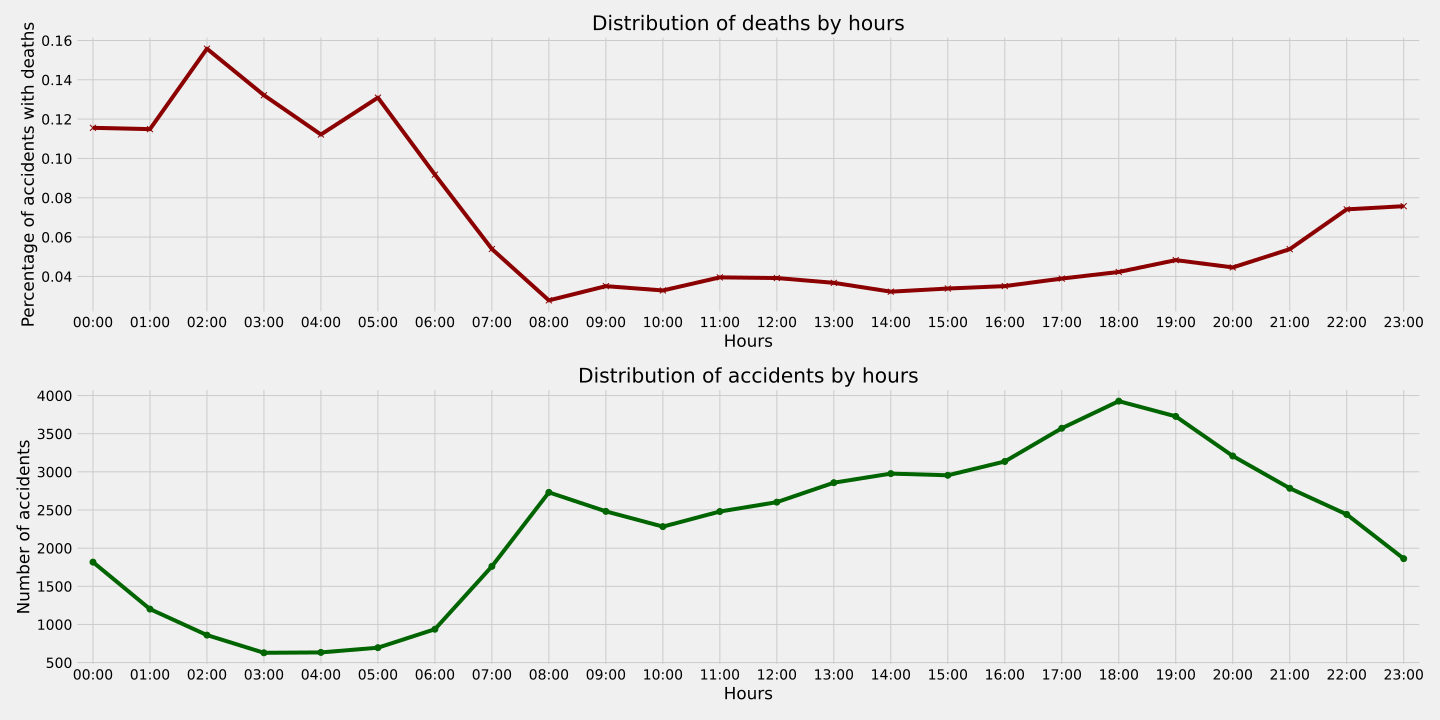
\includegraphics[width=0.8\textwidth]{../imgs/pdf_files/ts_distributions.pdf}
	\caption{Distribution of deaths and accidents by daytime}
	\label{fig:ts_dist}
\end{figure}
\begin{figure}[htpb]
	\centering
	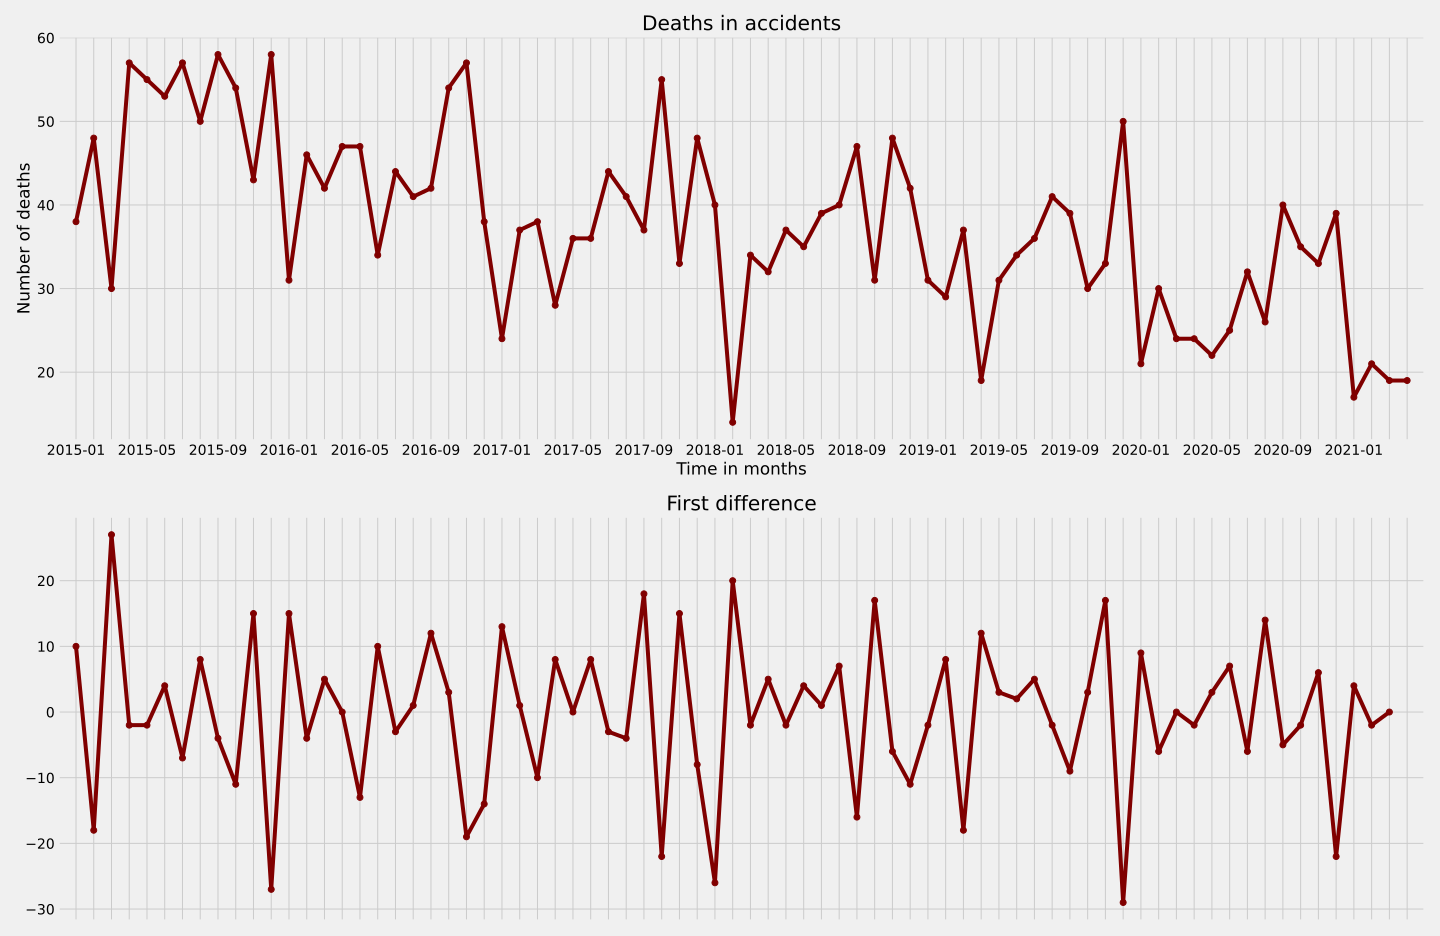
\includegraphics[width=0.8\textwidth]{../imgs/pdf_files/ts_death_first_diff.pdf}
	\caption{Number of deaths from 01.2015 till 04.2021}
	\label{fig:ts_death}
\end{figure}
